%- block legend
Kurt é um camaleão azul que gosta muito de matemática, computação e biologia celular. Atualmente ele está pesquisando um tipo peculiar de célula, que possui um nível de energia $K$ e é capaz de se multiplicar através de um processo que
ele batizou de Mitose Fibonáccica: a célula se divide em um conjunto de novas células cuja soma das energias é exatamente $K$, e cada uma dessas
novas células possui energia igual a um número de Fibonacci.
 
Usando sua expertise em computação, Kurt conseguiu programar a Mitose Fibonáccica de forma manipulada, fazendo com que o conjunto resultante tenha a
menor quantidade possível de células. Formalmente, ele obtém a decomposição de $K$ como soma da menor quantidade de números de Fibonacci
distintos que somam $K$.
 
Kurt possui $N$ células, cada uma com seu próprio valor energético $K_i$. Ele aplica a Mitose Fibonáccica manipulada em todas elas, de forma que cada célula
$i$ se divide em um novo conjunto de subcélulas como demonstrado na imagem a seguir:

\begin{center}
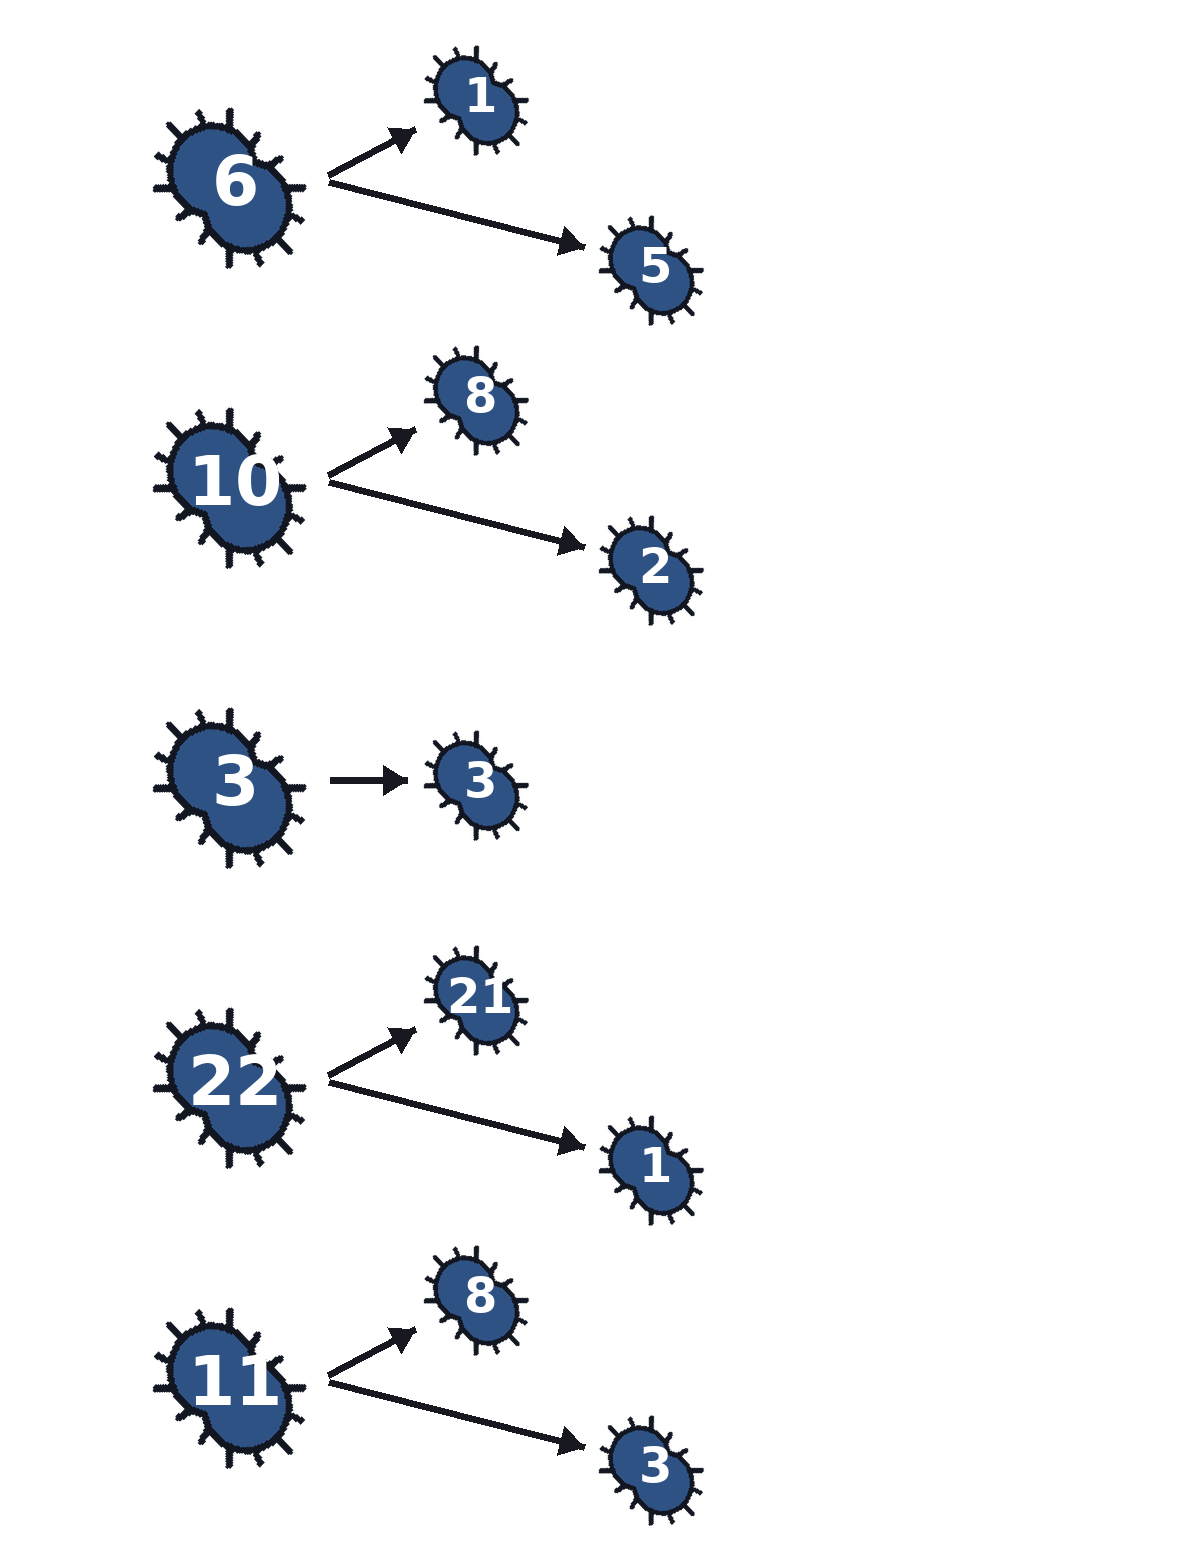
\includegraphics[scale=0.18]{mitose.png}
\end{center}
 
Como o resultado gerou muitos conjuntos pequenos, Kurt decidiu:
 
\begin{enumerate}
    \item Manter todas as subcélulas derivadas de uma mesma célula original
    $i$ em um único conjunto;
    \item Unir dois conjuntos sempre que eles possuírem pelo menos uma
    subcélula com o mesmo valor energético em comum.
\end{enumerate}
 
Depois dessas operações, Kurt quer saber qual é o conjunto com a maior quantidade de células com valores energéticos distintos. 

%- endblock

%- block input
A primeira linha contém um único inteiro $N$ ($1 \leq N \leq 10^5$). A quantidade de células que
Kurt possui.
 
A segunda linha contém $N$ inteiros $K_1, K_2, \ldots, K_N$ ($1 \leq K_i \leq 10^{18}$), os valores
energéticos de cada célula. É garantido que todo $K_i$ dado na entrada pode ser
escrito como a soma de um conjunto de números de Fibonacci.
%- endblock

%- block output
Imprima duas linhas:

Na primeira linha, a maior quantidade de valores energéticos distintos encontrado em um único conjunto.

Na segunda linha, os valores energéticos distintos desse conjunto, em ordem crescente, separados por espaço. Caso haja empate entre dois ou mais conjuntos com a maior quantidade de valores distintos, deve-se escolher o conjunto que
contiver a célula de menor valor energético.
%- endblock

%- block explanation_0
Neste exemplo, ilustrado na imagem anterior, os conjuntos de células com valor $K$ inicial $6$ e $22$ tem o uma célula com valor $1$ em comum, logo passam a formar um conjunto de tamanho $3 = [1, 5, 21]$.

E os conjuntos de células com valores energéticos iniciais $3$ e $11$ possuem uma célula com valor $3$ em comum e os conjuntos das células com valores energéticos iniciais iguais a $10$ e $11$ possuem uma célula com valor $8$ em comum, logo passam a formar um conjunto de tamanho $3 = [2, 3, 8]$.

Como ambos conjuntos formados tem tamanho $3$, o critério de desempate pelo conjunto com menor valor é o $[1, 5, 21]$.
%- endblock

%- block explanation_1
Neste exemplo todas as $N$ células já possuem seu valor enegético um número de fibonacci, logo o menor conjunto de números de fibonacci cuja a soma sejá $K_i$ são eles mesmos, então obtemos $4$ conjuntos de tamanho $1$,
e pelo critério de desempate, o $2$ possuí o menor valor energético.
%- endblock

%- block editorial
Usamos o Teorema de Zeckendorf: todo inteiro $K$ tem uma
única decomposição em Fibonaccis não consecutivos, e ela é justamente a
decomposição com a menor quantidade de termos possível. Ela é obtida de
forma gulosa, subtraindo sempre o maior Fibonacci $\le K$.

Como $K \le 10^{18}$, existem apenas $87$ Fibonaccis possíveis. Para cada
$K_i$, decompomos e unimos utilizando a estrutura de Disjoint-Set Union(DSU) nos termos consecutivos da
decomposição, marcando o tamanho do maior conjunto formado. Como os Fibonaccis são nós fixos e compartilhados entre
todas as decomposições, um valor repetido em dois $K_i$ diferentes já une os dois conjuntos automaticamente.
 
Ao final, percorremos o conjunto de todos os $87$ Fibonaccis em ordem
crescente e retornamos o primeiro (menor) cujo tamanho de componente é igual
a o maior conjunto — isso já resolve o desempate pelo menor valor.

Referência para o Teorema de Zeckendorf: \url{https://planetmath.org/zeckendorfstheorem}
Referência para o DSU: \url{https://cp-algorithms.com/data_structures/disjoint_set_union.html}
 
Complexidade: $O(N)$
%- endblock
